\part{Analysis and Implementation}

\chapter{Techniques and Wireless Tools}

\section{Introduction}

This section describes several possibilities a network can be set up and ways to infiltrate each type of network. All network types described that are not encrypted are illegal. As described in section \ref{sec:laws} it is not allowed to operate a network that does not take care of the security of the transferred data.

The second part of this section shows an evaluation of the most common wireless scanners. Additionally, some tools to break a WEP key are evaluated. Finally, the state of the art of wireless intrusion detection systems (WIDS) is shown.

\section{Open Networks with DHCP}

This type of network is the easiest to infiltrate. It is often installed by a person who does not care about security and wants the maximum amount of simplicity. The access point is used out of the box and remains unconfigured. It broadcasts beacon frames which contain the needed SSID to associate to the network. After associating to the access point an IP address can be obtained by using the DHCP service.

\begin{description}

\item [Linux:] The command to use the DHCP service on a network is
	{\em {\bf dhclient ethX}}
	where
	\begin{itemize}
		\item ethX is the name of the NIC which gets the new IP address
	\end{itemize}

\item [Windows:] No additional command is used. Windows takes care of assigning IP addresses in case a DHCP server is available

\end{description}

\section{Open Networks without DHCP}

In case no DHCP server is available on a network the IP information has to be gathered manually. This can either be done by trying the standard network IP addresses or by using wireless tools like Ethereal or Kismet.

\begin{description}

	\item [Standard IP addresses:]
		\cite{ipv4} shows the three standard IP address ranges for private 
		LANs. These ranges include:

	\begin{itemize}
		\item 192.168.0.0/16 (private network of class C)
		\item 172.16.0.0/12 (private network of class B)
		\item 10.0.0.0/8 (private network of class A)
	\end{itemize}

	\item [Tools:]
		Several tools like Ethereal or Kismet (see also section \ref{sec:wireless_scanners}) simplify the search for the correct IP address range of a network. When using Ethereal some frames have to be captured and the IP address of one client gives in most cases enough information to guess a valid IP address, the IP range and the address of the gateway. Kismet goes one step further and shows this information automatically after receiving data frames.

\end{description}

\section{Open Networks with ACLs}

As mentioned earlier, most access points offer the possibility to administrate ACLs which are also called {\em white lists}. These lists contain MAC addresses of valid stations that are allowed to connect to a network. If a station has a MAC address which is not listed in the ACL, it is blocked by the access point and its association request is denied.

Since a MAC address can be spoofed easily it is a matter of seconds to fool the access point by giving the wireless NIC a MAC address of a valid user:

\begin{description}

\item [Linux:] The command to change the MAC address of a NIC is

	{\em {\bf ifconfig ethX hw ether 00:AA:BB:CC:DD:EE}}

	where
	\begin{itemize}
		\item ethX is the name of the NIC the cracker wants to spoof
		\item 00:AA:BB:CC:DD:EE is the new MAC address of the NIC
	\end{itemize}
	
	In order to reset the MAC address of the NIC to the original one the cracker has to bring it down and up again by using the commands
	
	{\em {\bf ifconfig ethX down}} \\
	{\em {\bf ifconfig ethX up}}
	
\item [Windows:] There exist several tools to change the MAC address
	of a NIC named SMAC\footnote{A trial version of SMAC is available at:
	http://www.klcconsulting.net/smac/} or MacShift\footnote{MacShift is available at: http://devices.natetrue.com/macshift/}	

\end{description}


\section{Cloaked Networks}

Networks that are in hidden mode are hard to detect because the access point does not send out beacon frames which include the SSID. Additionally, it does not respond to probe requests in which the SSID field is not set.

One thing a cracker can do is to wait for an association of a legitimate user, capture the probe request frame sent and retrieve the SSID which is set in the request.

In case an intruder is aware of users that are currently connected to a cloaked network it is possible to speed up the process of waiting for an association of a new client: The only thing a cracker has to do is to send a disassociation request with the source address of a legitimate user which is currently connected to the network. The access point disassociates this station. Finally, the station realises that it was disconnected and reconnects automatically by sending a new association request.

\section{Encrypted Networks}

A network that is encrypted can also be infiltrated easily in case WEP is used. Depending on the encryption technique used it is a matter of hours, days or it is practically impossible to break into a network.

The following techniques to attack a WEP or WPA protected network are also described in \cite[p.60-62]{wlan_sicherheit} and \cite[p.130]{wlan_sicherheit}.

\subsection*{WEP Attacks}

\subsubsection{Brute Force}

This technique can be used for every encryption method and will always produce the correct result in case information about the plaintext is available. The idea is to try to decrypt an encrypted packet with all possible keys. The problem with this approach is that it takes a lot of time until the correct key is found. As a consequence this technique only makes sense in case a short key is used.

\subsubsection{Dictionary Attack}

The idea of a dictionary attack is the same as in a brute force attack. The only difference is that in a dictionary attack a predefined set of possible keys are tested instead of all possible ones. That means for example all words of an English dictionary serve as possible keys. In case the password used in a wireless network is an English word the correct key can be found faster than when using brute force since less keys have to be tested. The success of such an attack highly depends on the password chosen by the network administrator.

\subsubsection{FMS}

Based on the paper \cite{rc4weak} an attack was created to break the WEP key. It is named after its authors named {\bf F}luhrer, {\bf M}antin and {\bf S}hamir. The weakness focuses on the weak initialisation vectors (IVs) of RC4 which is used in WEP. There exist approximately 9000 of $2^{24}$ which have to be considered as insecure and can be used to perform the attack. As a consequence a lot of packets have to be captured. Additionally, manufacturers try to avoid to create weak IVs in their hardware which increases the number of packets needed. That means in detail that five to ten million (or even more) encrypted packets have to be captured before the attack succeeds. \cite[p.61f]{wlan_sicherheit}

\subsubsection{Improved FMS}

In 2002 David Hulton showed that it is possible to improve the FMS algorithm. This technique requires only 500.000 to 2.000.000 packets to break a WEP key successfully. For more information on the Improved FMS attack see \cite{improved_fms}.

\subsubsection{Statistical Cryptanalysis}

Currently the fastest way to break a WEP key was found by a hacker named KoreK. His method does not depend on weak IVs as it is the case in the techniques described above. The basis for this attack is the number of unique IVs. The number of needed packets to break a 128-bit WEP key lies somewhere around 500.000 to 1.000.000 packets. According to \cite[p.62]{wlan_sicherheit} KoreK did not describe the attack in papers or articles.

\subsection*{WPA Attack}

WPA is, compared to WEP, very robust \cite[p.129]{wlan_sicherheit} and as a consequence much harder to break. Nevertheless there exist possibilities to attack. The most common one is to run an offline attack by first capturing some frames and then perform a dictionary attack. Again, the success of such an attack depends on the password chosen by the network administrator.

\section{Wireless Scanners}
\label{sec:wireless_scanners}

The following section gives a brief overview of the most common wireless scanners including Netstumbler and Kismet.

\subsection*{Netstumbler}

Netstumbler is probably the most famous wireless scanner for Windows. It was written in 2001  by Marius Milner.

\pagebreak

The main features of Netstumbler include:

%\begin{spacing}{0.5}

\begin{itemize}
	\addtolength{\itemsep}{-1.5ex}

	\item \ac{GUI} based
	\item Graphical presentation of the signal strength and noise values
	\item Filtering of different types of wireless networks
    \item Active scanning\footnote{See section \ref{sec:active_passive_scanning} for details}
	\item \ac{GPS} support
	\item Support for Aironet, Hermes and Prism based NICs
	\item Save networks found in binary and proprietary NS1 file (Network Stumbler file)
	\item Export to readable text file
\end{itemize}

%\end{spacing}

Figure \ref{netstumbler} shows a screenshot of Netstumbler at work. The left frame groups all wireless networks found into different sections. These sections let a user group all networks found into different categories like showing only all encrypted networks, showing all infrastructure networks, etc.

\begin{figure}[htbp]
	\vspace{1.5em}
	\begin{center}
		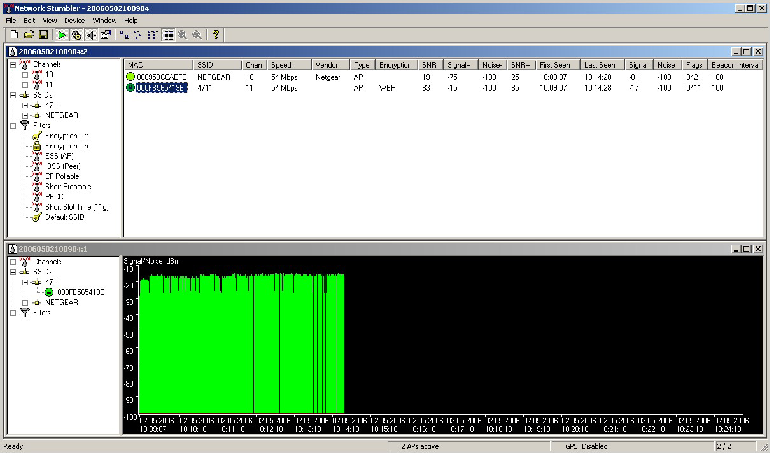
\includegraphics[width=1.0\columnwidth]{graphics/Netstumbler}
	\end{center}
	\vspace{-1em}
	\caption{The Netstumbler GUI}
	\vspace{1.5em}
	\label{netstumbler}
\end{figure}

\pagebreak

On the right side detailed information about a network is shown. See also \cite{netstumbler_columns}.

\begin{description}
	\addtolength{\itemsep}{-1.5ex}

	\item[MAC:] The MAC address of the network
	\item[SSID:] The name of the network
	\item[Channel:] The channel the network uses
	\item[Speed:] The maximum speed of the network in MBit/s
	\item[Vendor:] Netstumbler identifies vendors of networking technology by comparing the first three octets of the MAC address of an access point with a predefined database that contains vendors.\footnote{A list including the mapping between MAC address and vendor name can be found at: http://standards.ieee.org/regauth/oui/oui.txt}
	\item[Type:] Describes the type of the network. A possible value can either be {\em AP} (infrastructure BSS) or {\em Peer} (IBSS)
	\item[Encryption:] Shows whether a network is WEP protected or not
	\item[Signal to Noise Ratio (\ac{SNR}):] This value indicates the offset between the signal strength and the noise. The higher the difference the better it is for the quality of the connection \cite{snr}
	\item[SNR+:] The best SNR value of an AP found during a scan
	\item[Signal:] The current signal strength of an AP
	\item[Signal+:] The highest signal strength found during a scan
	\item[Noise:] The current noise value
	\item[Noise-:] The lowest noise value found during a scan
	\item[First Seen:] The time an AP was discovered
	\item[Last Seen:] The last time a frame was received by an AP
	\item[IP Addr and Subnet:] Shows IP address range and the subnet of a wireless network
	\item[Latitude and Longitude:] Information received by a GPS antenna
	\item[Beacon Interval:] The interval the AP or peer uses to send out beacon frames
	\item[Flags:] Shows the capabilities of an AP in hexadecimal notation. For detailed information about possible values see \cite[p.51]{80211standard}.
\end{description}

At the bottom of the window a two dimensional graph is presented which shows the SNR of a network.

\subsection*{Kismet}

Another wireless scanner for Linux is Kismet, written by Mike Kershaw. Due to the fact that it is a passive scanner (see section \ref{sec:active_passive_scanning} for details) the wireless NIC used to capture frames has to be able to be put into monitor mode. Since the wireless NIC can capture all frames that are sent through the air it is also possible to detect cloaked networks by scanning and dissecting data frames. Because it detects (almost) every network Kismet is very often used by wardrivers.

The main features of Kismet are (see also \cite{kismet_readme} and \cite{guide_to_wardriving}):

\begin{itemize}
	\addtolength{\itemsep}{-1.5ex}

	\item GUI based on Ncurses\footnote{Ncurses is a graphic library for Linux which creates windows and panels on a console using coloured dashes. For more information on Ncurses visit its project homepage at: http://www.gnu.org/software/ncurses/ncurses.html.}
    \item Passive scanning
	\item GPS support
	\item Channel hopping support
	\item It supports "any wireless card which
    supports raw monitoring (rfmon) mode, and can sniff 802.11b, 802.11a, and
    802.11g traffic." \cite{kismet_readme}
	\item Automatically logs access points to \ac{XML}, \ac{CSV} and GPS files
	\item Automatically logs raw data to pcap files
	\item Network IP range detection
	\item Detection of default access point configurations
	\item Manufacturer identification of access points and wireless NICs
	\item Show MAC addresses of clients that are connected to a network
	\item Present a statistic of a network
\end{itemize}

\begin{figure}[htbp]
	\begin{center}
		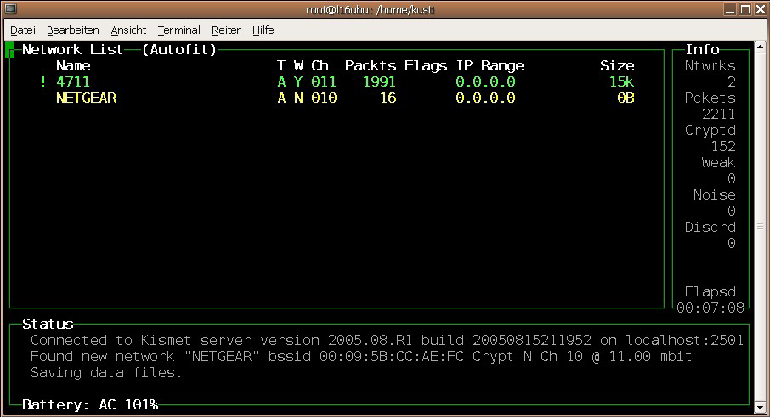
\includegraphics[width=1.0\columnwidth]{graphics/Kismet}
	\end{center}
	\vspace{-1em}
	\caption{The Kismet GUI}
	\label{kismet}
\end{figure}

Figure \ref{kismet} shows a screenshot of Kismet at work. The main window named {\em Network List} shows detailed information about networks found:

\begin{description}
	\addtolength{\itemsep}{-1.5ex}

	\item[Name:] The SSID of the network
	\item[T:] Type of the network. Possible values include {\em P} (probe requested network), {\em A} (infrastructure BSS) and {\em H} (IBSS)
	\item[W:] Encryption type used in the network. Values can be {\em N} for no encryption, {\em Y} for WEP encryption and {\em O} for any other encryption used
	\item[Ch:] Specifies the channel the networks uses
	\item[Packts:] The number of packets that are sent over the network
	\item[Flags:] Gives information about characteristics of the network. Possible values include {\em F} (the AP is unconfigured. That means it uses well-known standard password(s) and IP range) and {\em D} (DHCP traffic found)
	\item[IP Range:] Specifies which IP addresses are used in a network
	\item[Size:] The amount of data that is sent over a network
\end{description}

The frame on the right side named {\em Info} gives general information about networks and data:

\begin{description}
	\addtolength{\itemsep}{-1.5ex}

	\item[Ntwrks:] The number of networks found
	\item[Pckets:] The number of packets captured
	\item[Cryptd:] The number of encrypted packets captured
	\item[Weak:] The number of packets that contain a weak IV
	\item[Noise:] The number of packets that are scrambled due to too high noise values
	\item[Discrd:] The number of discarded packets
	\item[Elapsd:] The time Kismet is up and running
\end{description}

The panel on the bottom of the page named {\em Status} shows general information about Kismet and the logs created by the WIDS that is included in Kismet.

\section{WEP Cracking Tools}

The following section gives a brief overview of tools which are capable of breaking a WEP key using different techniques.

\subsection*{AirSnort}

Probably one of the most famous WEP cracking tool for Windows and Linux is AirSnort. It was developed in 2001 by Jeremy Bruestle and Blake Hegerle, and implements the FMS attack.

\begin{figure}[htbp]
	\vspace{1.5em}
	\begin{center}
		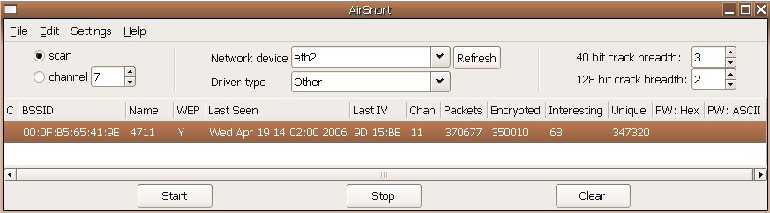
\includegraphics[width=1.0\columnwidth]{graphics/Airsnort}
	\end{center}
	\vspace{-1em}
	\caption{The AirSnort GUI}
	\vspace{1.5em}
	\label{airsnort}
\end{figure}

As figure \ref{airsnort} shows it is GUI based and offers several configuration options. To break a WEP key it is either possible to scan the network in real time (a cracking attempt is done each time ten weak IVs are captured) or load a \ac{pcap file} with WEP encrypted packets. Additional options include the cracking breadth for 64 and 128 bit keys. The higher the breadth rate the more time it takes to break a WEP key but the higher the probability to find the correct one. A result in the {\em PW: Hex} and {\em PW: ASCII} column does not mean that the correct key was found. The documentation of AirSnort states that it uses a probabilistic approach which means that it tries to guess the correct key.

As it is shown in \cite[p.61f]{wlan_sicherheit} AirSnort requires at least five million encrypted packets to break a WEP key. Depending on the captured data and the amount of weak IVs this value can also exceed the ten million mark.

In case a GPS device is available AirSnort also supports GPS. That offers the possibility to log the current position of the capturing entity.

\subsection*{Dwepcrack}

In 2002 a hacker named h1kari created a console based implementation of the Improved FMS attack and named it Dwepcrack which runs solely under Linux.

In addition to the Improved FMS attack it implements an advanced brute force attack which is especially well suited for 64 bit WEP keys. It manages to break down the key length from $2^{40}$ to $2^{21}$ possible keys. That makes it possible to perform a brute force attack in a reasonable amount of time. See also \cite{wep_dead_1}.

\subsection*{WepLab}

"WepLab is a tool designed to teach how WEP works, what different vulnerabilities it has, and how they can be used in practice to break a WEP protected wireless network. ... The author has tried to leave the source code as clear as possible, running away from optimizations that would obfuscate it." \cite{weplab} WepLab was developed in 2004 by Jose Ignacio Sanchez Martin alias Topo[LB] for Windows and Linux.

The main features of WepLab include:

\begin{itemize}
	\addtolength{\itemsep}{-1.5ex}

	\item Analyse a pcap file and show relevant information like the number of captured packets and the number of unique IVs
	\item Perform a brute force attack to break a WEP key
	\item Perform a dictionary attack to break a WEP key
	\item Perform a statistical cryptanalysis attack to break a WEP key
	\item Capture packets from a wireless NIC
	\item Specify the length of the WEP key (64 or 128 bit)
	\item Specify the amount of keys tested using the --perc option (default: 50). The higher this value the higher the probability to find the correct key but the longer the search takes
\end{itemize}

\subsection*{Aircrack}

Aircrack is an implementation of the statistical cryptanalysis attack. \cite{wep_dead_1} says that Aircrack provides the fastest and most effective attack currently available. It runs under Windows and Linux.

The main features of Aircrack include:

\begin{itemize}
	\addtolength{\itemsep}{-1.5ex}

	\item Perform a statistical cryptanalysis attack to break a WEP key
	\item Specify the length of the WEP key (64 or 128 bit)
	\item Perform a dictionary attack on a WPA-PSK protected network
	\item The so called {\em fudge factor} specifies the amount of keys tested. The higher this value the higher the probability to find the correct key but the longer the search takes
\end{itemize}

In addition to Aircrack some tools are delivered:

\begin{description}
	\item [802ether:] Creates an unencrypted pcap file out of a WEP encrypted one by specifying the source and destination pcap file and the WEP key used
	\item [airodump:] Captures packets of a wireless network and stores it in a pcap file. It is also possible to store only the unique IVs which are relevant for Aircrack
	\item [aireplay:] Performs an active WEP attack in order to guess the WEP key by injecting previously captured encrypted packets
\end{description}

\subsection*{Tests and Results}

A test has shown (see Appendix \ref{sec:aircrack_weplab}) that Aircrack and Weplab require at least 800.000 packets containing approximately 341.000 unique IVs to break a 64 bit WEP key definitely.

An interesting detail concerning the test result is that in some cases it was possible for Aircrack to break the WEP by using only 100.000 packets containing 40.832 unique IVs to find the correct key. The calculation took from one to three minutes depending on the fudge factor.

WepLab also found the correct WEP key by using only 400.000 packets with 167.740 unique IVs in less than five minutes.

These results indicate that the success to break a 64 bit WEP key mainly depends on three things:

\begin{description}
    \item[The amount of data:] As shown in the test Aircrack and WepLab succeeded in breaking the key as soon as they had enough data (800.000 packets with 341.000 unique IVs).
	\item[The captured data itself:] Both, Aircrack and WepLab, showed that it is possible to find the correct key in case less data is available.
	\item[Parameters:] WepLab found a correct key when using the value 70 for the --perc parameter but did not find it when using the values 50 or 90.
\end{description}

Another test which is illustrated in \cite[p.207-210]{wlan_sicherheit} presents a similar result. In this test it is shown that WepLab performs a little bit better than Aircrack when it comes to 64 bit WEP keys. Some exceptional results in the Aircrack test also show that the success to break a WEP key does not only depend on the amount of captured data.

\section{State of the Art WIDS}

The following section gives a brief overview of wireless intrusion detection systems which are freely available on the Internet.

\subsection*{AirSnare}

AirSnare is a freely available WIDS for Windows. It was created in 2002 by Jay L. DeBoer and Thomas Bruinsma. Figure \ref{airsnare} shows AirSnare at work.

\begin{figure}[htbp]
	\vspace{1.5em}
	\begin{center}
		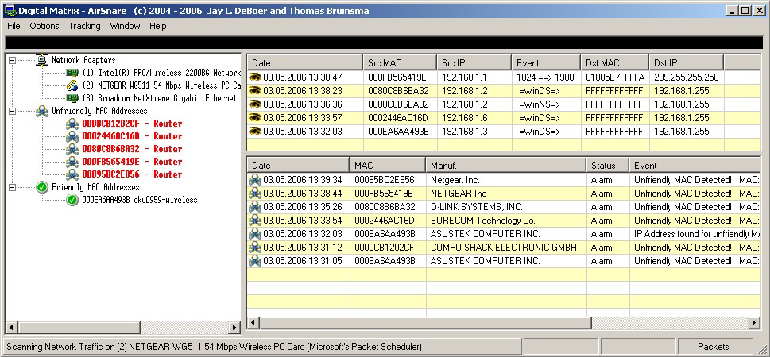
\includegraphics[width=1.0\columnwidth]{graphics/Airsnare}
	\end{center}
	\vspace{-1em}
	\caption{The AirSnare GUI}
	\vspace{1.5em}
	\label{airsnare}
\end{figure}

After starting AirSnare and choosing one wireless NIC that scans the traffic AirSnare displays information about MAC and IP addresses, and events that occurred. As soon as a new MAC address is found it is marked as {\em Unfriendly MAC Address}. All these clients are monitored. Each MAC address found can be set into the {\em Trusted MAC Address} state so that no more alarms are triggered by that MAC address.  In addition to the MAC addresses the IP address of each client is shown.

Another feature of AirSnare is that it displays DHCP requests captured. This is useful to identify malicious users. In case no DHCP server is available but a DHCP request is captured then it is possible that a malicious user tries to gather information about a network.

AirSnare also provides the {\em net send} command for Windows which makes it possible to send a message to every client that runs the messenger service. This service is enabled by default.\footnote{For more information about the Windows messenger service see also http://support.microsoft.com/default.aspx?scid=KB;EN-US;168893}

In case an unfriendly MAC address is found an automatic mail can be sent to the network administrator to inform about uncontrolled behaviour in the network.

\subsection*{Wireless Snort}

Wireless Snort is the extension to the Snort program which is used in wired networks and works under Windows and Linux. This tool is written by Andrew Lockhard in 2003.

One aspect that makes Wireless Snort very powerful is the possibility to create custom rules. These rules are used to detect particular WLAN packets that are sent in the network.\footnote{An example for a rule could be to detect all association requests that come from a certain MAC address} Depending on the definition of the rule different actions can be taken. For more information about defining rules and using actions see \cite{wireless_snort_rules}. The most important actions include:

\begin{description}
	\addtolength{\itemsep}{-1.5ex}
    \item[alert:] This action generates an alert and then logs the packet
	\item[log:] This action only logs the packet
	\item[pass:] This action ignores the packet
\end{description}

In addition to defining custom rules Wireless Snort also provides the ability to detect DoS attacks and Netstumbler fingerprints.

\subsection*{Kismet}

As we have seen in the previous section Kismet is a powerful wireless scanner. In addition to that it can also be used as a WIDS. Table \ref{kismetalerts}  shows all alerts Kismet can throw. The list of alerts and descriptions is also available in \cite{kismet_readme}. All events thrown are displayed in the {\em Status} panel shown in figure \ref{kismet}.

\begin{table}[htbp]
	\begin{center}
		\begin{tabular}{|p{150pt}|p{200pt}|}
		\hline
		\bf{Name}&\bf{Description}\\
		\hline
		Netstumbler probe requests&In an attempt to disclose the SSID of a network, Netstumbler sends out unique packets\\
		\hline
		Deauthenticate/Disassociate Flood&By spoofing disassociate or deauthenticate packets, arbitrary (or all) clients can be disconnected from a
network\\
		\hline
		Lucent link test&Lucent/Orinoco/Proxim/Agere provide site survey 
software. Kismet detects the usage of these tools\\
		\hline
		Wellenreiter SSID brute force attempt&Wellenreiter attempts to use a dictionary to brute-force a hidden SSID.  Between each probe attempt it resets the card to probe for 'this\_is\_used\_for\_wellenreiter'\\
		\hline
		Previously detected AP changing to a new channel&Man-in-the-middle attacks attempt to direct users to a fake AP on another channel\\
		\hline
		Broadcast disconnect/ deauthenticate&Many attacks use a broadcast disassociate or deauthenticate to disconnect all users on a network, 
either to redirect them to a new fake network or do cause a denial of service or disclose a cloaked SSID\\
		\hline
		SSID of 'airjack'&The AirJack tool sets the initial SSID to 'airjack'\\
		\hline
		Clients probing for networks, being accepted by that network, and continuing to probe for networks&'Active' or 'Firmware' network scanning tools work by letting the card probe for any network and recording those that respond\\
		\hline
		Traffic from a source within 10 seconds of a disassociation&A host which legitimately disassociates or deauthenticates from a network should not be 
exchanging data immediately thereafter\\
		\hline
		Probe response packet with 0 length SSID tagged parameter&Many firmware versions from different manufacturers have a fatal error when they receive a probe response with a 0 length SSID tagged parameter\\
		\hline
		Invalid BSS timestamps indicative of an access point being spoofed&The BSS timestamp sent with beacons and some probe frames cannot be spoofed with standard firmware or drivers even when forging raw frames\\
		\hline
		\end{tabular}
	\end{center}
	\caption{WIDS alerts Kismet can throw}
	\label{kismetalerts}
\end{table}

Kismet can also be used as a distributed WIDS. It manages drones which send their captured data to a dedicated server which then checks for a possible threat.

\subsection*{WIDZ}

In 2003 Mark Osborne designed and implemented a tool named WIDZ. He says that the tool is only a {\em proof of concept} to show insecurities in wireless networks. \cite{widz_design} It runs solely under Linux.

WIDZ detects basic attacks like \ac{rogue AP}s, active scanners and flood attacks. It is possible to create white and black lists of MAC addresses and a white list for SSIDs. Additionally, a user can create alert scripts that are run whenever WIDZ triggers an alarm.

According to \cite[p.3f]{widz_design} WIDZ is divided into two different modules:

\begin{description}
    \item[AP monitor:] This module is capable of identifying \ac{bogus AP}s\footnote{See glossary} and \ac{unauthorised AP}s\footnote{See glossary}. Both types of attacks are identified by comparing simple text files that contain MAC addresses with the MAC addresses found
\pagebreak
	\item[Traffic monitor:] Since not all threats can be detected by managing text files this module deals with identifying other type of attacks. The most severe attacks that can be recognised by WIDZ are {\em probe monitoring}\footnote{Probe monitoring means detecting active scanners by searching for probe requests where the SSID is not set} and {\em flood detection}

\end{description}

\subsection*{Additional Remarks}

Despite the possibility to operate a WIDS that monitors a whole network there exists a problem that all tools presented have in common. A wireless network can use 11 different channels. In order to detect rogue APs\footnote{See glossary} it is necessary to monitor all channels at the same time. This can either be done by running a WIDS for every single channel which is an expensive solution or to use one single WIDS which performs channel hopping. The problem with the latter solution is that the WIDS might miss traffic that is sent during the periods it does not listen to a certain channel. In the worst case an attack is performed exactly at that time.

\subsection*{Conclusion}

Table \ref{wids_compare} shows a brief comparison of all Linux based WIDS presented above. This evaluation is taken and adopted from \cite{wlan_sicherheit}.

\begin{table}[htbp]
	\vspace{1.5em}
	\begin{center}
		\begin{tabular}{|p{80pt}|p{80pt}|p{80pt}|p{80pt}|}
		\hline
		\bf{Type}&\bf{Wireless Snort}&\bf{Kismet}&\bf{WIDZ}\\
		\hline
		DoS&yes&yes&yes\\
		\hline
		Active attack&yes&yes&yes\\
		\hline
		Rogue AP&no&not automated&yes\\
		\hline
		Re-injection&no&no&no\\
		\hline
		Distributed&yes&yes&no\\
		\hline
		\end{tabular}
	\end{center}
	\vspace{-1em}
	\caption{Feature comparison of different WIDS}
	\vspace{1.5em}
	\label{wids_compare}
\end{table}

All WIDSs evaluated are freely available on the Internet and each of them has its advantages and drawbacks. Kismet and Wireless Snort seem to be very sophisticated because they also allow the creation of distributed systems with drones that collect data and send it to a server. Another advantage of Kismet is that the installation is easy and it can be used without handling difficult configuration files. On the other hand Wireless Snort allows the system to store the gathered information in a database. The actual decision which WIDS to choose  depends on the needs of the network administrator.
